\documentclass[a4paper]{article}

\input{math_commands.tex}

\usepackage[final, nonatbib]{ofu_xai_2022}

\usepackage[utf8]{inputenc}
\usepackage[T1]{fontenc}
\usepackage{hyperref}
\usepackage{url}
\usepackage{booktabs}
\usepackage{amsfonts}
\usepackage{nicefrac}
\usepackage{microtype}
\usepackage{xcolor}
\usepackage{graphicx}
\usepackage{multirow}

\usepackage[round]{natbib}

\title{Domain Generalization for In-the-Wild Waste Classification: \\
Measuring, Diagnosing, and Mitigating the Gap Between Clean and Real-World Data}

\author{%
  Esmaeil Molapour \\
  Otto-Friedrich University of Bamberg\\
  96049 Bamberg, Germany\\
  \texttt{esmaeil.molapour@stud.uni-bamberg.de} \\[0.3cm]
  Seminar: xAI-Proj-M \\
  Degree: M.Sc. Software Systems Science \\
  \AND
  Ashly Varghese \quad Khaled Ibrahim \quad Khawar Khan \\
  Otto-Friedrich University of Bamberg
}

\begin{document}

\maketitle

\begin{abstract}
Models for waste classification are almost always trained on clean, object-centric photographs, yet they get deployed somewhere much messier: real bins and real landfills, full of clutter, crushed objects, and inconsistent lighting. This project measures that gap directly. Three architectures (ResNet-50, EfficientNet-B3, ViT-Small) were trained on 18{,}042 images from two clean-domain sources (TrashNet, GD12) and then tested zero-shot on RealWaste, a genuine landfill dataset that never appears in training. The result is a 35--42\% drop in balanced accuracy across all three models. Grad-CAM points to why: misclassified images are the ones where the model is attending to background clutter or printed text rather than the material itself. From there we tried three ways of closing the gap. Two of them backfired --- heavier synthetic augmentation and a third, more visually diverse training dataset both made out-of-distribution accuracy \emph{worse}. What did work was a smaller, more targeted change: dropping the noisiest class, switching to resize-padding, adding label smoothing, and introducing a border-background augmentation that leaves the object untouched and only varies the surrounding pixels. This pushed zero-shot RealWaste accuracy up to 64.5\% for ViT-Small, without the model ever seeing a single target-domain image. We also pushed the approach to its breaking point using TACO, a dataset of litter photographed in natural scenes rather than as isolated objects; accuracy collapsed to 33--39\% for every architecture equally, which we read as a task-structure boundary (object-centric classification versus in-context detection) rather than a further generalization failure. A calibration analysis (ECE, AUROC) turned up something we did not expect going in: accuracy and calibration are inversely related across architectures, with ViT-Small being the most accurate model and simultaneously the least trustworthy about its own confidence, while EfficientNet-B3 sits at the opposite end. An independently collected 170-image dataset, photographed by our own team, confirms the mitigation benefit for both CNNs but exposes a limitation specific to ViT-Small. Finally, Wilcoxon and McNemar tests confirm what the large-sample results suggest while appropriately holding back on the smaller-sample comparisons where the evidence is weaker.
\end{abstract}

\section{Introduction}
\label{sec:intro}

Automated waste sorting is one of the more practical applications of computer vision for recycling infrastructure, at least in principle. In practice, models trained on clean, catalog-style photographs tend to fail once they meet a real waste stream \citep{babe2025generalization, hossen2024reliable}. Part of the reason is well documented in the domain-adaptation literature: there is a gap between the \emph{source domain} used for training (well-lit, single object, uncluttered) and the \emph{target domain} encountered at deployment (crushed, dirty, cluttered, badly lit), and this gap remains a central open problem in applied waste classification \citep{abdu2022survey}.

Three questions shaped this project. How large is the domain gap, and does it depend on which architecture is used? What visual cues actually cause models to fail out-of-distribution, and can the standard toolbox --- more augmentation, more training data --- close the gap, or does it need something more targeted? And finally, if the gap can be closed for one kind of real-world data (object-centric photographs), does that success carry over to a structurally different kind of real-world data, such as litter photographed in context rather than isolated?

We address these questions through a systematic experimental pipeline spanning 38 logged experiments (Appendix~\ref{app:experiments}), covering baseline training, failure diagnosis via Grad-CAM \citep{selvaraju2017gradcam}, three mitigation strategies, a scope-boundary evaluation, an independently collected validation dataset, calibration analysis, and statistical significance testing.

\section{Related Work}
\label{sec:related}

Convolutional architectures such as ResNet \citep{He_2016_CVPR} and EfficientNet \citep{tan2019efficientnet} remain the dominant backbones for waste classification \citep{celik2025multilayer, sayem2025enhancing}, while transformer-based architectures \citep{dosovitskiy2021vit} have seen more limited application in this domain. \citet{babe2025generalization} specifically studied the generalization ability of foundation models for waste classification and reported substantial accuracy degradation under domain shift, consistent with our findings. \citet{arishi2025realtime} and \citet{hossen2024reliable} report strong in-distribution results but do not systematically test OOD generalization or mitigation strategies, which is the primary contribution of this work. We additionally draw on \citet{guo2017calibration} for calibration methodology (Section~\ref{sec:calibration}).

\section{Datasets}
\label{sec:datasets}

\paragraph{Training data.} We combine two clean-domain sources into a unified 6-class training set (cardboard, glass, metal, paper, plastic, trash), later simplified to 5 classes (Section~\ref{sec:redesign}): TrashNet (2{,}527 images, white-background studio photography) and GD12 (15{,}515 images, 12 original classes mapped to our 6; battery, biological waste, clothing, and shoes are mapped to \emph{trash} as non-recyclable general waste). This yields 18{,}042 training images, split 70/15/15 (train/val/test, seed 42).

\paragraph{Out-of-distribution test data.} RealWaste \citep{realwaste} contains 4{,}752 images of real landfill waste across 9 categories, mapped to our 6 (Miscellaneous Trash, Food Organics, Textile Trash, and Vegetation $\to$ trash). RealWaste is held out entirely from training in our primary experiments (Sections~\ref{sec:baseline}--\ref{sec:diagnosis}) to serve as a genuine zero-shot benchmark.

\paragraph{Scope-boundary test data.} TACO \citep{taco2020} consists of 1{,}500 photographs of litter in natural and urban scenes, annotated with 4{,}784 bounding boxes across 60 fine-grained categories. We map these to our 6 classes and crop each annotation into an individual image to construct a classification-format test set (Section~\ref{sec:taco}).

\paragraph{Own hard dataset.} To validate findings on an independently collected source, our team photographed 170 real-world waste items following an object-centric protocol (single item, filling the frame, genuine environmental clutter). The metal class (17 images) was excluded from evaluation after a diagnosed composition failure (small objects photographed against disproportionately large natural backgrounds; Section~\ref{sec:owndataset}), yielding 142 usable images across 4--5 classes depending on experimental configuration.

We use \emph{balanced accuracy} (mean per-class recall) throughout, as all datasets are class-imbalanced.

\section{Models and Training}
\label{sec:models}

We train three ImageNet-pretrained architectures, chosen to test whether generalization behavior depends on architectural inductive bias: \textbf{ResNet-50} \citep{He_2016_CVPR} (convolutional, local receptive fields, residual connections), \textbf{EfficientNet-B3} \citep{tan2019efficientnet} (compound-scaled convolutional network), and \textbf{ViT-Small/16} \citep{dosovitskiy2021vit} (patch-based self-attention, no convolutional locality prior). All models are fine-tuned for 20 epochs using AdamW (initial learning rate $1\times10^{-4}$, cosine annealing), weighted cross-entropy loss to address class imbalance, and standard ImageNet normalization.

\section{Baseline Results: The Domain Gap}
\label{sec:baseline}

\begin{table}[t]
\caption{In-distribution vs.\ zero-shot out-of-distribution (RealWaste) balanced accuracy, original 6-class setup.}
\label{tab:baseline}
\centering
\begin{tabular}{lccc}
\toprule
Model & In-Distribution & Zero-Shot OOD & Domain Gap \\
\midrule
ResNet-50 & 95.5\% & 60.0\% & $-$35.5 pts \\
EfficientNet-B3 & 96.0\% & 53.6\% & $-$42.4 pts \\
ViT-Small & 97.4\% & 62.2\% & $-$35.2 pts \\
\bottomrule
\end{tabular}
\end{table}

All three architectures achieve 95--97\% in-distribution balanced accuracy but drop by 35--42 percentage points when evaluated zero-shot on RealWaste (Table~\ref{tab:baseline}). ViT-Small generalizes best, EfficientNet-B3 worst; this ranking reproduces consistently across every subsequent zero-shot experiment in this work (Sections~\ref{sec:redesign}, \ref{sec:owndataset}), suggesting it reflects a genuine architectural property rather than experimental noise.

\section{Diagnosis: What Causes the Gap?}
\label{sec:diagnosis}

We use Grad-CAM \citep{selvaraju2017gradcam} to visualize which image regions drive each model's predictions. For ViT-Small, standard Grad-CAM is inapplicable since the architecture lacks convolutional feature maps; we use a patch-reshaping transform to recover a spatial attention map from the transformer's output sequence.

Across all three architectures, correct predictions are associated with activation concentrated on the object's surface and edges, while misclassifications are frequently associated with activation on background texture or printed text/logos rather than the object itself (Figure~\ref{fig:gradcam}). This indicates that models trained purely on clean-domain images learn source-domain surface shortcuts (background style, print) rather than generalizable material-level features. We additionally tested whether the heterogeneous \emph{trash} class (aggregating battery, biological waste, clothing, shoes, and other non-recyclables) was a primary driver of the gap by excluding it from scoring; balanced accuracy \emph{decreased}, since trash was consistently the models' best-performing class on RealWaste. This rules out label heterogeneity as the primary cause and is consistent with the surface-shortcut explanation.

\begin{figure}[t]
\centering
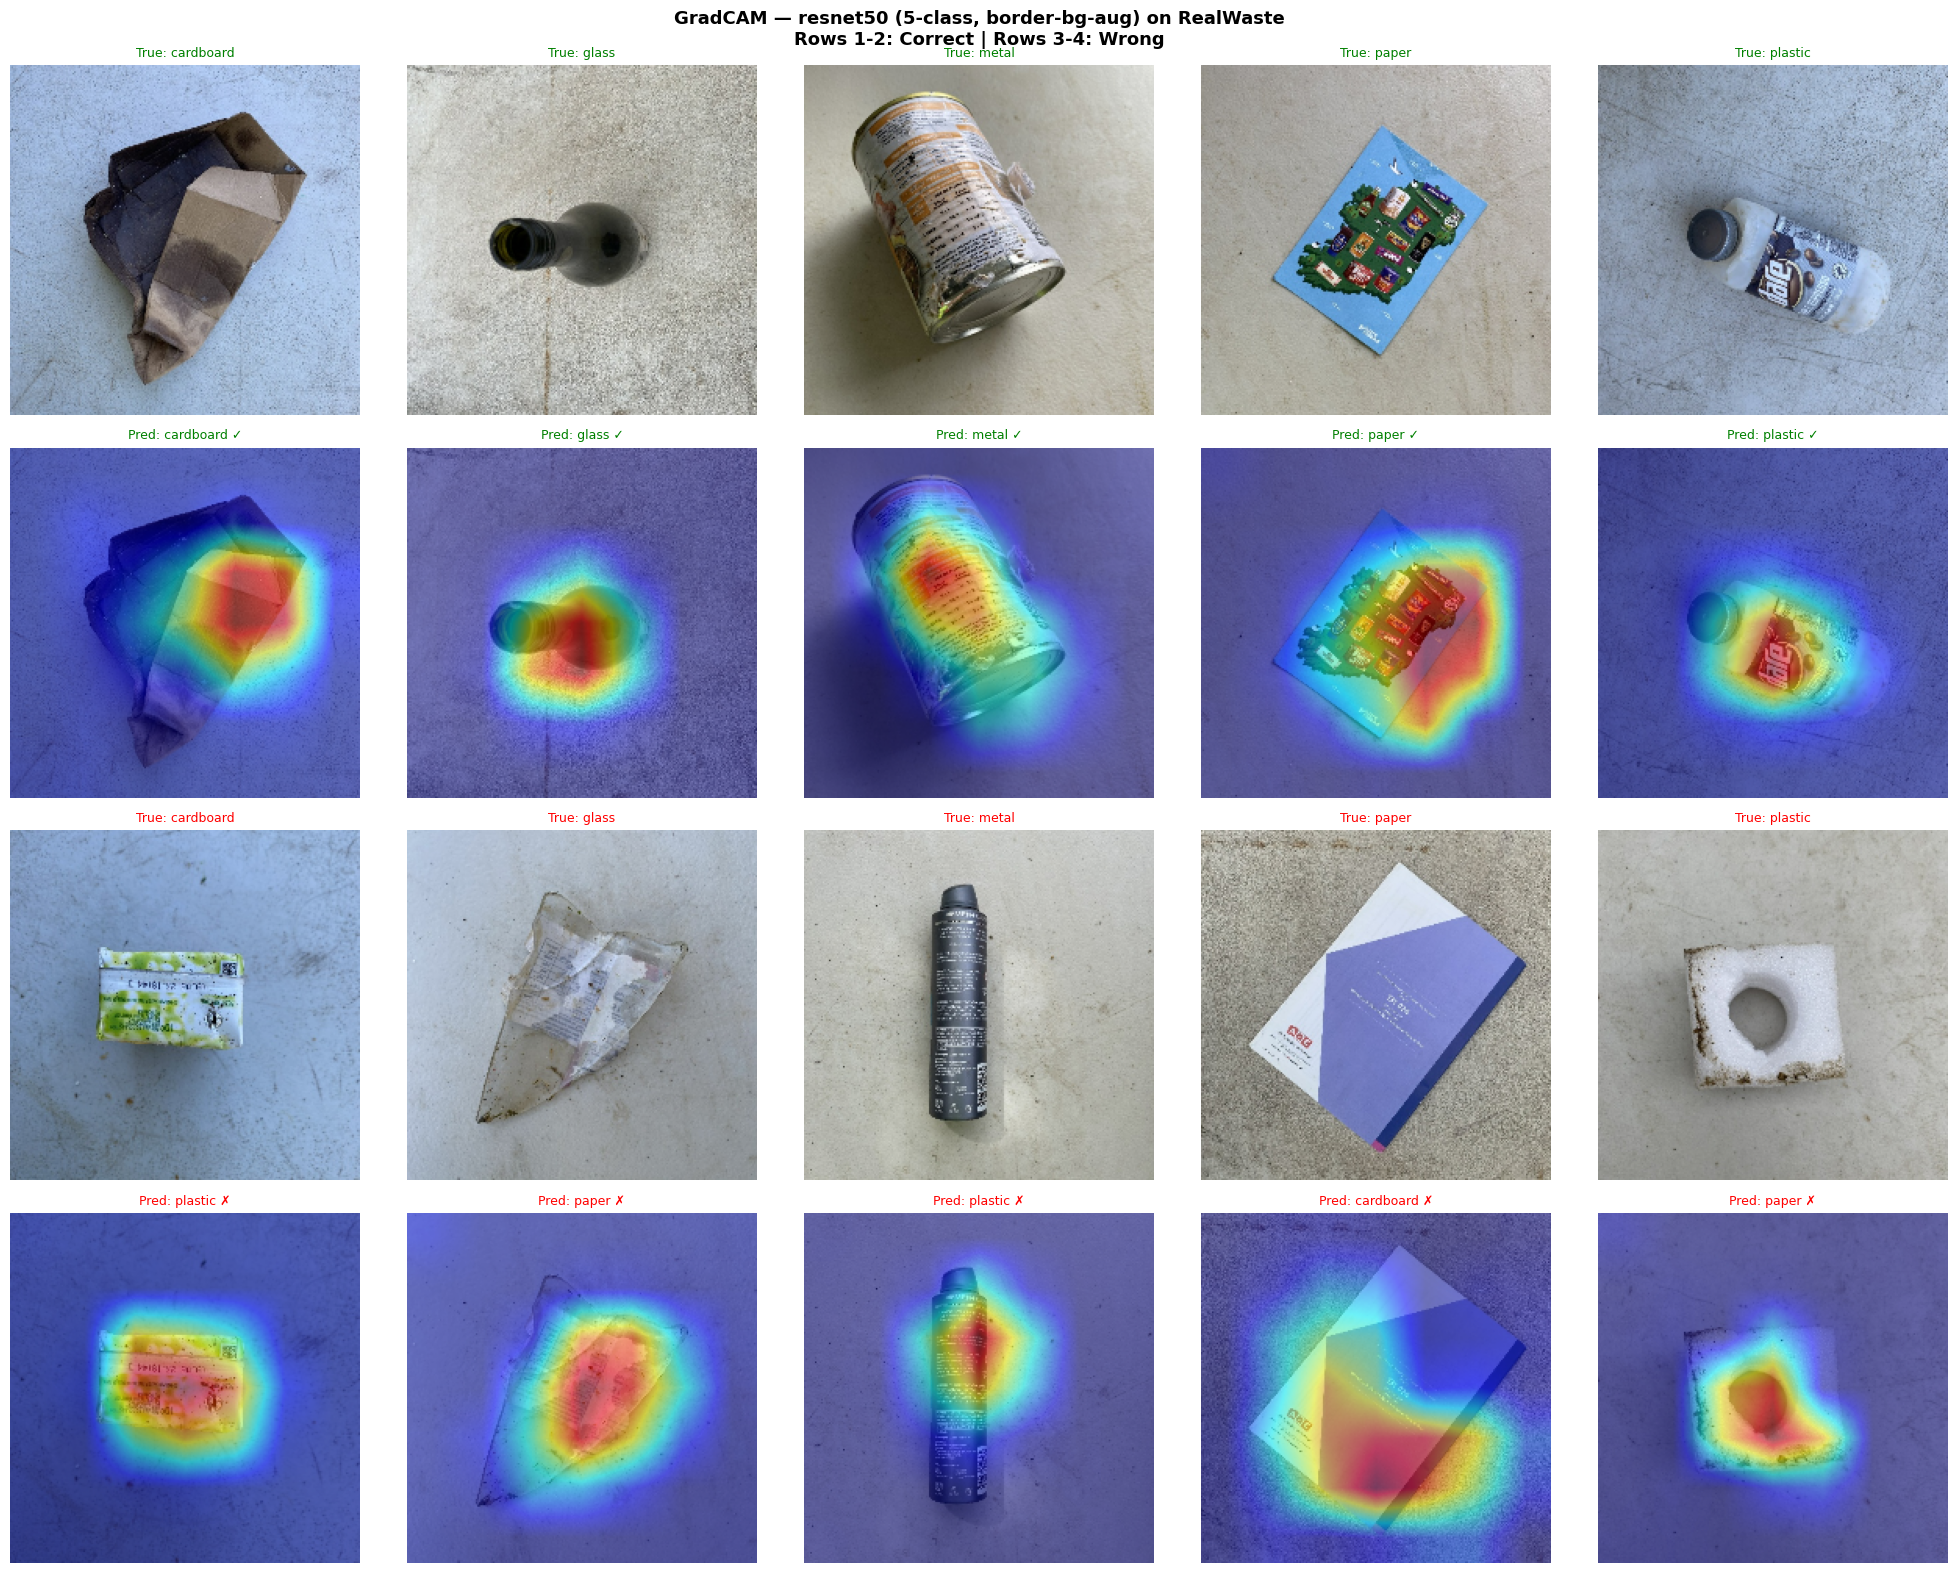
\includegraphics[width=0.98\linewidth]{figures/gradcam_resnet50_5class.png}
\caption{Grad-CAM visualizations for ResNet-50 (5-class, border-background-augmented model) on RealWaste. Top two rows: correct predictions, activation concentrated on the object. Bottom two rows: misclassifications, activation more diffuse or shifted toward surface content.}
\label{fig:gradcam}
\end{figure}

\section{Mitigation Strategies}
\label{sec:mitigation}

Three mitigation strategies were tried, each one a direct response to what the failure diagnosis above suggested.

\paragraph{Strategy 1: Heavier synthetic augmentation.} The first, most obvious idea was to make training harder: standard augmentation was swapped for a heavier pipeline (motion blur, shadows, occlusion, noise) meant to push training images closer to real-world conditions. In-distribution accuracy ticked up slightly (95.5\%$\to$97.4\% for ResNet-50), but zero-shot RealWaste accuracy went the wrong way (60.0\%$\to$57.0\%). The likely explanation is that this kind of augmentation just makes the model more confident about the source domain, without teaching it anything that actually transfers.

\paragraph{Strategy 2: Additional same-domain training data.} The second idea was more data, specifically a third public dataset (sumn2u, 12{,}259 images, 10 classes) merged into training. Despite the extra volume and nominally more varied backgrounds, zero-shot accuracy dropped again, to 56.4\%. On closer inspection, TrashNet, GD12, and sumn2u all turn out to be visually similar despite coming from different sources --- clean, single-object photography, essentially the same domain wearing different clothes. Adding more of that domain just gives the model more source-specific patterns to memorize, not more generalization. That failure is what motivated the redesign below.

\paragraph{Strategy 3 (redesigned pipeline): Border-background augmentation.}
\label{sec:redesign}
Following the diagnosis that models over-rely on background cues, we redesign the pipeline with five changes evaluated jointly and then ablated: (i) simplification to 5 classes (cardboard, glass, metal, paper, plastic), removing the heterogeneous trash class entirely; (ii) a resize-and-pad transform replacing center-cropping, to avoid discarding off-center objects; (iii) label smoothing (0.1) and increased weight decay ($2\times10^{-2}$) to reduce overconfidence; (iv) checkpoint selection by validation balanced accuracy rather than validation loss; (v) \emph{border-background augmentation}: rather than segmenting the foreground object (found unreliable; see Appendix~\ref{app:segmentation}), we replace only the outer border of each training image with a synthetic textured background, leaving the object region untouched. Crucially, RealWaste is not used in training at any point for this strategy---it remains a genuine zero-shot test set throughout.

\begin{table}[t]
\caption{Ablation of border-background augmentation (ResNet-50, 5-class, all other components held constant), and full rollout to all architectures.}
\label{tab:ablation}
\centering
\begin{tabular}{lccc}
\toprule
Model & Without Aug.\ (Control) & With Border-BG Aug. & $\Delta$ \\
\midrule
ResNet-50 & 56.5\% & 58.0\% & +1.5 pts \\
EfficientNet-B3 & --- & 53.8\% & --- \\
ViT-Small ($\eta{=}1\text{e-}4$) & --- & 63.0\% & --- \\
ViT-Small ($\eta{=}2\text{e-}5$) & --- & 64.5\% & --- \\
\bottomrule
\end{tabular}
\end{table}

Table~\ref{tab:ablation} shows a controlled ablation isolating the augmentation's effect: with every other factor held constant, border-background augmentation improves zero-shot RealWaste accuracy by 1.5 points for ResNet-50---a small but genuine effect, and notably the \emph{opposite} direction from the generic augmentation in Strategy 1, supporting our diagnosis that the type of augmentation matters more than its presence. Rolling this configuration out to all three architectures, ViT-Small achieves 64.5\% zero-shot accuracy (after a learning-rate sensitivity check reduced $\eta$ from $1\times10^{-4}$ to $2\times10^{-5}$; Appendix~\ref{app:lr}), the best zero-shot result obtained in this work without any target-domain data.

\paragraph{Domain adaptation variant.} We separately evaluated a fourth strategy in which 15\% of RealWaste (712 images) is added to training, with the remaining 85\% (4{,}040 images) held out for evaluation. This produced substantially larger gains (76.4\%, 79.9\%, 81.6\% for ResNet-50, EfficientNet-B3, and ViT-Small respectively), but we emphasize that this experiment answers a \emph{different research question}: limited-supervision domain adaptation rather than zero-shot generalization. The held-out 85\% was never seen in training, but because some RealWaste data informed training, these results are not directly comparable to the zero-shot figures elsewhere in this paper and are reported as a separate, clearly labeled protocol (Appendix~\ref{app:adaptation}).

\section{Scope Boundary: TACO}
\label{sec:taco}

To test how far the improvements above generalize, we evaluate the border-background-augmented models on TACO, a structurally different type of real-world data. Accuracy collapses to 33--39\% across all three architectures, despite the same checkpoints achieving 58--65\% on RealWaste. Notably, all three architectures converge to a nearly identical accuracy on TACO (33.3\%, 34.1\%, 33.8\%)---a pattern inconsistent with a generalization failure (which would typically show architecture-dependent variation) and consistent with a task-structure mismatch. We investigated crop dimensions and found 42\% of TACO bounding-box crops fall below $100\times100$ pixels; filtering to larger crops recovers only a small improvement (to 38--39\%). We conclude that TACO represents \emph{in-context litter detection} (small, partial objects within complex natural scenes) rather than the \emph{object-centric classification} task our models are trained for, and that closing this gap requires a detection-then-classification architecture (e.g., YOLO) rather than further classifier tuning. We treat this as a documented scope boundary rather than a deficiency of the proposed mitigation.

\section{Independent Validation: Own Dataset}
\label{sec:owndataset}

\begin{table}[t]
\caption{Zero-shot balanced accuracy on our independently collected dataset (5-class configuration, metal excluded; 142 images), compared to RealWaste.}
\label{tab:owndataset}
\centering
\begin{tabular}{lcc}
\toprule
Model & RealWaste & Own Dataset \\
\midrule
ResNet-50 & 58.0\% & 45.2\% \\
EfficientNet-B3 & 53.8\% & 41.2\% \\
ViT-Small & 63.0\% & 55.3\% \\
\bottomrule
\end{tabular}
\end{table}

To confirm findings are not specific to RealWaste, we evaluate the same border-background-augmented checkpoints on our independently collected dataset (Table~\ref{tab:owndataset}). The architecture ranking (ViT $>$ ResNet $>$ EfficientNet) reproduces exactly, the fourth consecutive confirmation of this ordering across the project. Absolute accuracy is lower than on RealWaste, consistent with our dataset representing a harder or differently distributed real-world source. The metal class was excluded after diagnosis revealed a photography protocol failure---small objects (e.g., bottle caps, tent pegs) photographed against disproportionately large natural backgrounds, structurally resembling the TACO failure mode---illustrating that even carefully collected validation data is sensitive to composition, and reinforcing the object-centric vs.\ in-context distinction identified in Section~\ref{sec:taco}.

\section{Calibration Analysis}
\label{sec:calibration}

Following \citet{guo2017calibration}, we compute Expected Calibration Error (ECE) and use max-softmax confidence as an OOD-detection signal (AUROC), evaluating whether models' confidence estimates are trustworthy under distribution shift.

\begin{table}[t]
\caption{Calibration metrics on RealWaste (OOD). Overconfidence gap = mean confidence $-$ accuracy.}
\label{tab:calibration}
\centering
\begin{tabular}{lcccc}
\toprule
Model & OOD Accuracy & OOD ECE & Overconf.\ Gap & OOD-Detection AUROC \\
\midrule
ResNet-50 & 60.2\% & 0.132 & +0.131 & 0.757 \\
EfficientNet-B3 & 55.4\% & 0.047 & +0.046 & \textbf{0.885} \\
ViT-Small & \textbf{65.9\%} & 0.153 & +0.153 & 0.666 \\
\bottomrule
\end{tabular}
\end{table}

Table~\ref{tab:calibration} reveals a striking inverse relationship: ViT-Small, the most accurate model, is the \emph{worst} calibrated and least able to signal its own uncertainty (lowest AUROC), while EfficientNet-B3, the least accurate model, is the \emph{best} calibrated. This pattern reproduces on our own dataset (Appendix~\ref{app:calibration}), confirming it is a robust architectural property rather than a dataset-specific artifact. The reliability diagram (Figure~\ref{fig:reliability}) shows all three models are overconfident in the mid-to-high confidence range (0.3--0.85) but slightly underconfident at low confidence, refining the simple ``models are overconfident'' narrative. Practically, this suggests EfficientNet-B3 may be preferable in deployment settings where flagging uncertain predictions for human review matters as much as raw accuracy.

\begin{figure}[t]
\centering
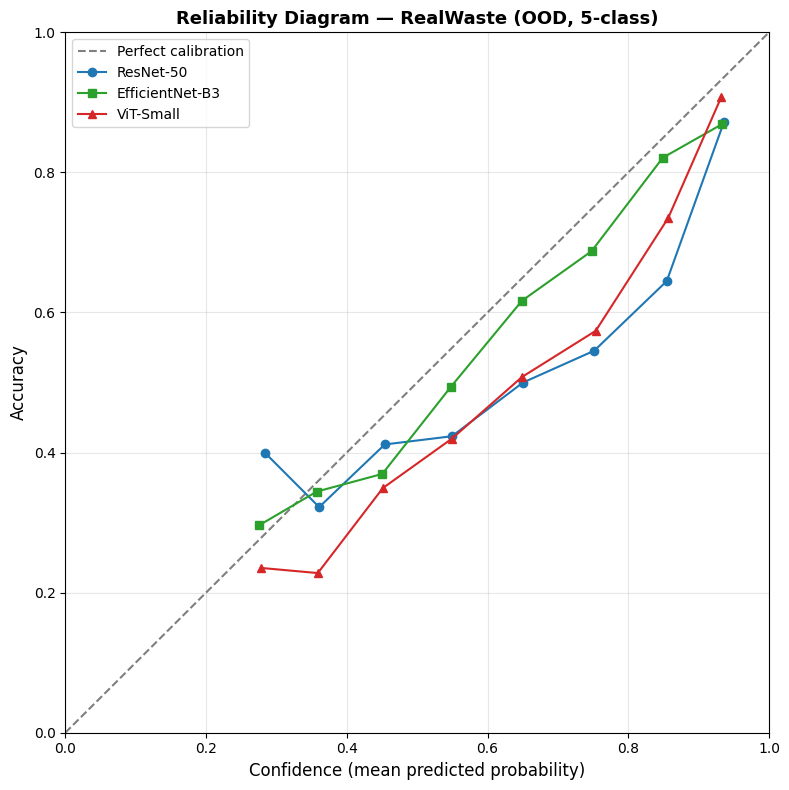
\includegraphics[width=0.65\linewidth]{figures/reliability_diagram.png}
\caption{Reliability diagram on RealWaste. All models lie below the diagonal (overconfident) for confidence $>0.4$; ViT-Small deviates furthest, EfficientNet-B3 tracks closest to perfect calibration.}
\label{fig:reliability}
\end{figure}

\section{Statistical Significance}
\label{sec:stats}

We test pairwise architecture differences using both the Wilcoxon signed-rank test and McNemar's test (the latter being the statistically appropriate test for paired binary classification outcomes) on per-image correctness. On RealWaste ($n=3{,}092$), all pairwise differences are significant ($p<0.001$) by both tests. On our own dataset ($n=142$), results are more nuanced: ResNet-50 vs.\ EfficientNet-B3 is not significant by either test; EfficientNet-B3 vs.\ ViT-Small is significant by both; ResNet-50 vs.\ ViT-Small is significant by Wilcoxon ($p=0.042$) but \emph{not} by McNemar's test ($p=0.057$). We report the more rigorous McNemar result and explicitly note that the own-dataset ViT-vs-ResNet advantage, while directionally consistent with all other results, should be interpreted as suggestive rather than statistically confirmed given the small sample size.

\section{Results Summary}
\label{sec:summary}

\begin{figure}[t]
\centering
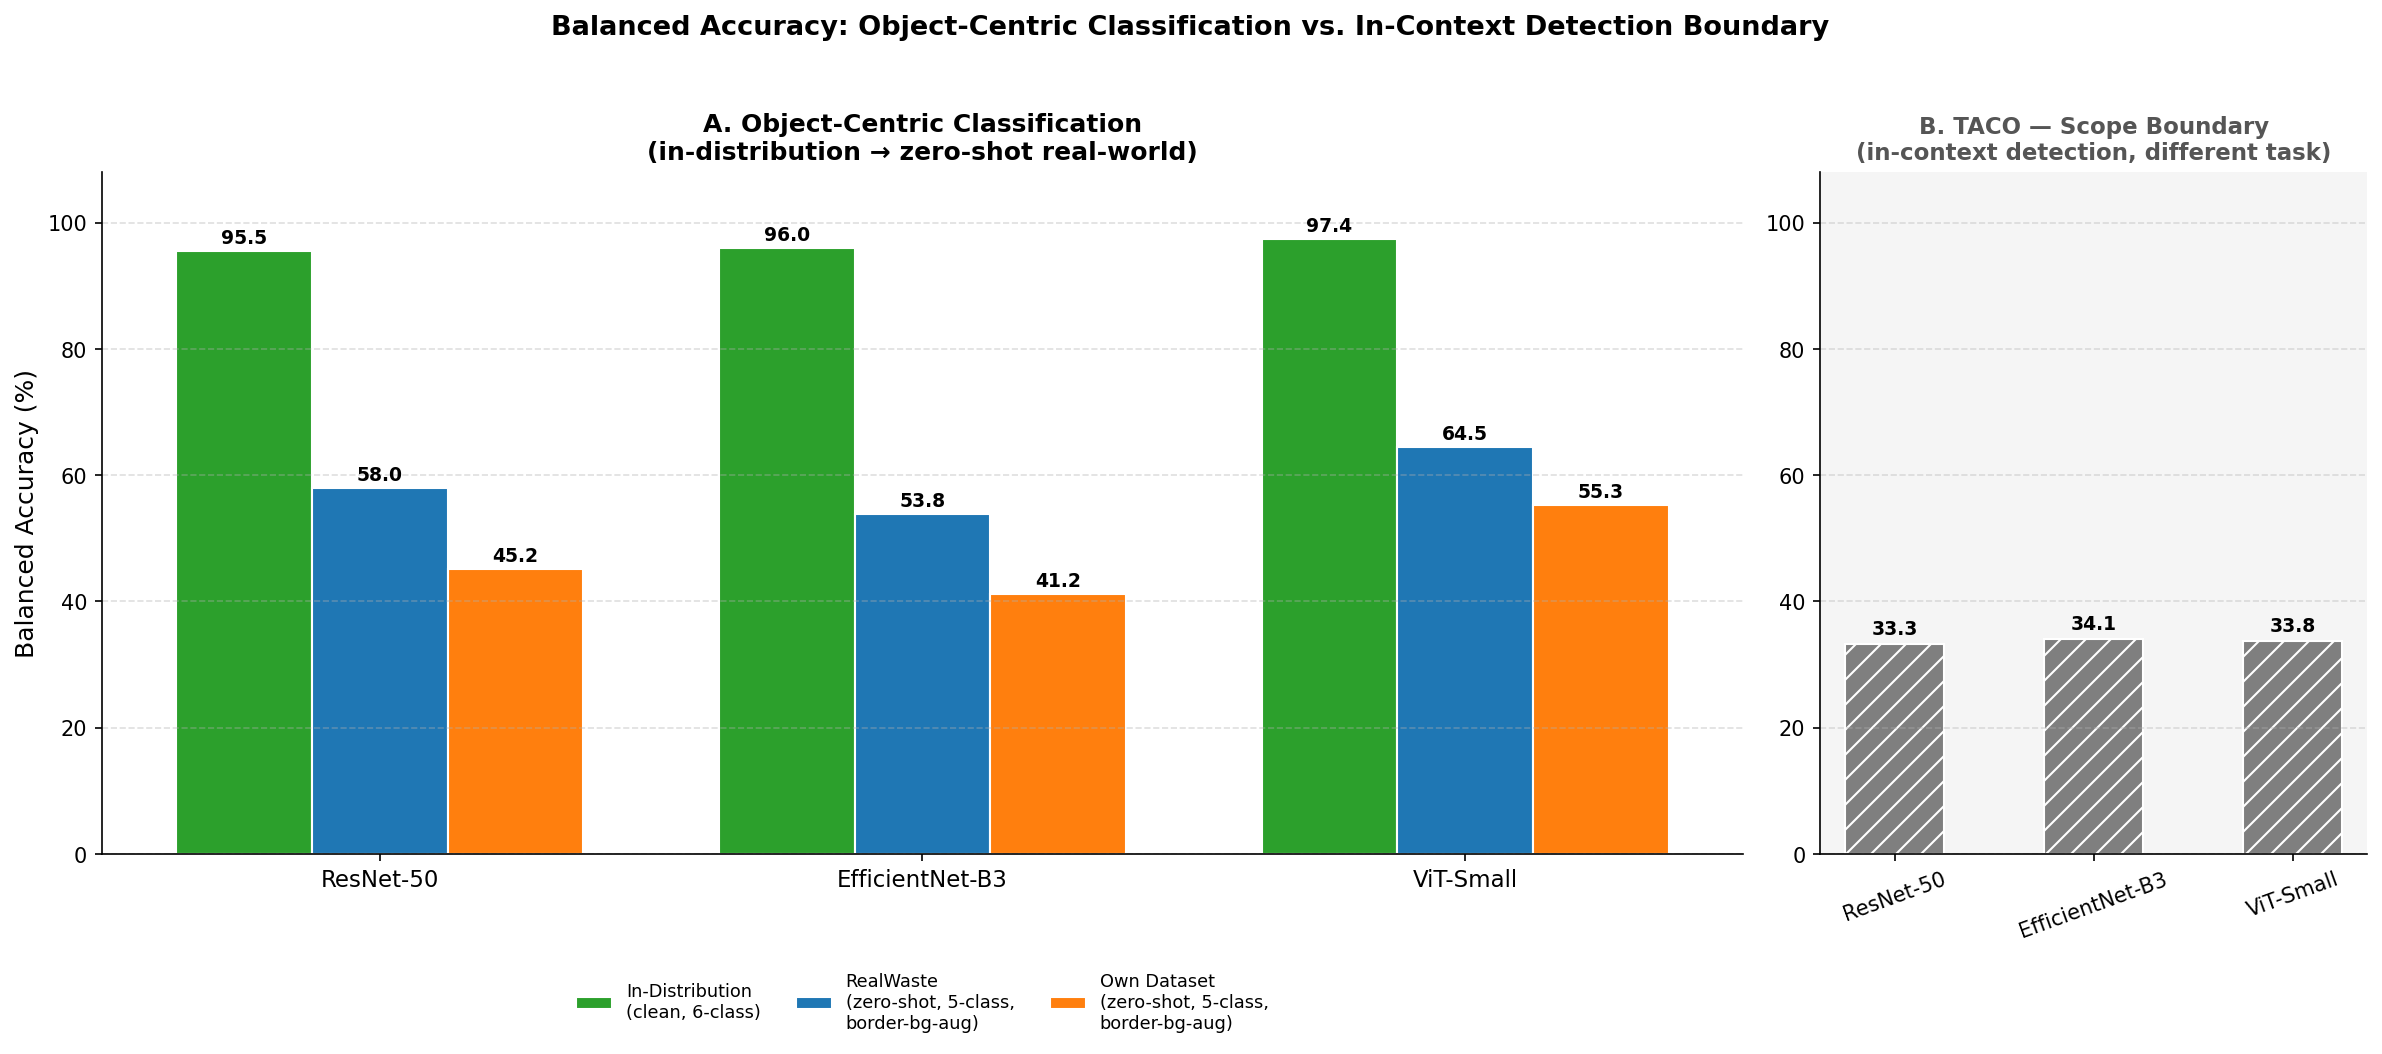
\includegraphics[width=\linewidth]{figures/results_bar_chart_v2.png}
\caption{Balanced accuracy across test conditions. Panel A: object-centric classification (in-distribution through zero-shot real-world transfer). Panel B: TACO, shown separately as it represents a structurally different task (in-context detection) rather than a comparable failure.}
\label{fig:summary}
\end{figure}

Figure~\ref{fig:summary} summarizes results across all test conditions. We deliberately separate TACO into its own panel to avoid the misleading impression that it represents a fourth point of comparable failure on the same task; as established in Section~\ref{sec:taco}, it measures a different problem entirely.

\section{Discussion and Limitations}
\label{sec:discussion}

Our central finding is that \emph{data type matters more than data quantity or synthetic diversity} for closing the domain gap in waste classification: two strategies that added substantial training data (Sections~\ref{sec:mitigation}, Strategies 1--2) both worsened OOD accuracy, while a targeted, low-cost augmentation change (border-background replacement) produced a small but genuine and statistically-grounded improvement without any target-domain data. The larger gains from limited-supervision domain adaptation (Appendix~\ref{app:adaptation}) further support this: even a small quantity of genuinely target-domain data outperforms large quantities of same-domain data.

Several limitations warrant statement. First, the domain-adaptation experiment (Appendix~\ref{app:adaptation}) necessarily uses a portion of RealWaste in training; we have taken care to report this as a separate protocol from our zero-shot results throughout, per methodological feedback received during project supervision. Second, our own dataset (142--170 images) is small, and Section~\ref{sec:stats} shows that not all architecture comparisons on it reach statistical significance. Third, addressing the TACO scope boundary would require an object-detection architecture, which is outside the scope of this classification-focused project. Fourth, we did not test domain-adversarial training objectives or frozen-backbone fine-tuning, both of which are plausible further mitigation strategies motivated by our findings.

\section{Conclusion}
\label{sec:conclusion}

We provide a systematic empirical study of domain generalization for waste classification, characterized by five main findings: (1) a large, consistent 35--42\% zero-shot domain gap exists across three distinct architectures; (2) common mitigation strategies (heavier augmentation, additional same-domain data) reliably \emph{worsen} this gap; (3) a targeted augmentation addressing the diagnosed failure mode (background reliance) yields a small, statistically grounded, zero-shot improvement; (4) an accuracy/calibration trade-off exists at the architecture level, reproduced across two independent OOD datasets; and (5) a genuine task-structure scope boundary separates object-centric classification from in-context litter detection. Future work should pursue object-detection-based approaches for in-context litter and explore domain-adversarial training objectives building on the diagnosis established here.

\section*{Acknowledgments}
We thank Sebastian Doerrich for supervision and detailed methodological feedback throughout this project, including guidance on evaluation protocol separation and dataset scope.

\newpage
\section*{References}
\small
\bibliography{bibliography}
\bibliographystyle{abbrvnat}

%%%%%%%%%%%%%%%%%%%%%%%%%%%%%%%%%%%%%%%%%%%%%%%%%%%%%%%%%%%%%%%%%%%%%%%%%%%%%%%%%%%%%%%%%%%%%%%%%%%%
%% Declaration of Authorship
%%%%%%%%%%%%%%%%%%%%%%%%%%%%%%%%%%%%%%%%%%%%%%%%%%%%%%%%%%%%%%%%%%%%%%%%%%%%%%%%%%%%%%%%%%%%%%%%%%%%
\newpage
\section*{Declaration of Authorship}
Ich erkl\"{a}re hiermit gem\"{a}\ss{} \S{} 9 Abs. 12 APO, dass ich die vorstehende Seminararbeit selbstst\"{a}ndig verfasst und keine anderen als die angegebenen Quellen und Hilfsmittel benutzt habe. Des Weiteren erkl\"{a}re ich, dass die digitale Fassung der gedruckten Ausfertigung der Seminararbeit ausnahmslos in Inhalt und Wortlaut entspricht und zur Kenntnis genommen wurde, dass diese digitale Fassung einer durch Software unterst\"{u}tzten, anonymisierten Pr\"{u}fung auf Plagiate unterzogen werden kann.

\vspace{2\baselineskip}
Bamberg, \today

\rule[0.5em]{14em}{0.5pt} \hspace{0.25\linewidth}\rule[0.5em]{14em}{0.5pt}
\vspace{1em}

\hspace{4em} (Ort, Datum) \hspace{0.51\linewidth} (Unterschrift)

\section*{Individual Contributions}
\textbf{Esmaeil Molapour}: data pipeline construction and dataset curation, all model training, baseline and zero-shot evaluation, Grad-CAM diagnosis, design and execution of all mitigation experiments, TACO pipeline and scope-boundary analysis, own-dataset collection protocol and evaluation, calibration analysis, statistical testing, and report writing. \textbf{Khaled Ibrahim}: evaluation methodology planning, contribution to calibration metric design. \textbf{Khawar Khan}: experiment tracking infrastructure, architecture literature review. \textbf{Ashly Varghese}: contribution to early augmentation experiment design.

\appendix

\section{Full Experiment Log Summary}
\label{app:experiments}
This project logged 38 experiments (EXP001--EXP035, with sub-experiments), tracked in \texttt{experiment\_log.py} in the accompanying code repository. Table~\ref{tab:explog} summarizes the major experimental phases; full per-experiment notes, hyperparameters, and results are available in the repository.

\begin{table}[h]
\caption{Major experimental phases.}
\label{tab:explog}
\centering
\small
\begin{tabular}{ll}
\toprule
Phase & Experiments \\
\midrule
Baseline training \& class-weight fix & EXP001--EXP008 \\
Zero-shot OOD baseline (RealWaste) & EXP009--EXP011 \\
Mitigation: augmentation, 3rd dataset & EXP012--EXP015 \\
Trash-class diagnostic & EXP016 \\
Domain adaptation (15\% RealWaste) & EXP017--EXP019 \\
TACO scope-boundary evaluation & EXP020--EXP023 \\
Own dataset evaluation \& diagnosis & EXP024--EXP027 \\
5-class redesign \& border-bg augmentation & EXP028--EXP029 \\
Calibration analysis & EXP030, EXP032 \\
Own dataset re-evaluation (5-class) & EXP031 \\
ViT learning-rate check & EXP033 \\
Statistical significance testing & EXP034--EXP035 \\
\bottomrule
\end{tabular}
\end{table}

\section{Foreground Segmentation Attempt}
\label{app:segmentation}
An initial attempt at background augmentation used GrabCut-based foreground segmentation to precisely isolate objects before background replacement. Visual inspection revealed this approach frequently misclassified parts of the object itself (particularly light-colored interior regions of open cardboard boxes) as background, corrupting training images. This was identified and discarded prior to any training run, in favor of the safer border-only replacement strategy described in Section~\ref{sec:redesign}.

\section{Domain Adaptation Protocol Detail}
\label{app:adaptation}

\begin{table}[h]
\caption{Domain adaptation results: 15\% of RealWaste (712 images) added to training, evaluated on the remaining 85\% (4{,}040 images, held out).}
\label{tab:adaptation}
\centering
\begin{tabular}{lccc}
\toprule
Model & Zero-Shot (Table~\ref{tab:baseline}) & Domain Adaptation & $\Delta$ \\
\midrule
ResNet-50 & 60.0\% & 76.4\% & +16.4 pts \\
EfficientNet-B3 & 53.6\% & 79.9\% & +26.3 pts \\
ViT-Small & 62.2\% & 81.6\% & +19.4 pts \\
\bottomrule
\end{tabular}
\end{table}

We emphasize again that these results answer a different question (limited-supervision domain adaptation) than our zero-shot results and are not directly comparable to them, per feedback received during project supervision regarding evaluation protocol separation.

\section{ViT Learning Rate Sensitivity}
\label{app:lr}
Motivated by the sensitivity of transformer architectures to learning rate, we re-trained ViT-Small at $\eta=2\times10^{-5}$ (vs.\ the shared $\eta=1\times10^{-4}$ used for all architectures in Section~\ref{sec:redesign}). This improved zero-shot RealWaste accuracy from 63.0\% to 64.5\%---a modest but genuine gain, indicating the original learning rate was mildly suboptimal for this architecture without overturning the central finding that ViT-Small is the strongest zero-shot generalizer of the three architectures tested.

\section{Own-Dataset Calibration}
\label{app:calibration}
\begin{table}[h]
\caption{Calibration metrics on the own dataset (OOD), confirming Table~\ref{tab:calibration}.}
\centering
\begin{tabular}{lccc}
\toprule
Model & OOD Accuracy & Overconf.\ Gap & OOD-Detection AUROC \\
\midrule
ResNet-50 & 43.7\% & +0.252 & 0.873 \\
EfficientNet-B3 & 36.6\% & +0.167 & \textbf{0.923} \\
ViT-Small & 54.9\% & +0.193 & 0.790 \\
\bottomrule
\end{tabular}
\end{table}
The AUROC ranking (EfficientNet-B3 $>$ ResNet-50 $>$ ViT-Small) reproduces exactly from RealWaste, confirming the accuracy/calibration trade-off identified in Section~\ref{sec:calibration} is not a RealWaste-specific artifact.

\section{Confusion Analysis}
\label{app:confusion}
\begin{figure}[h]
\centering
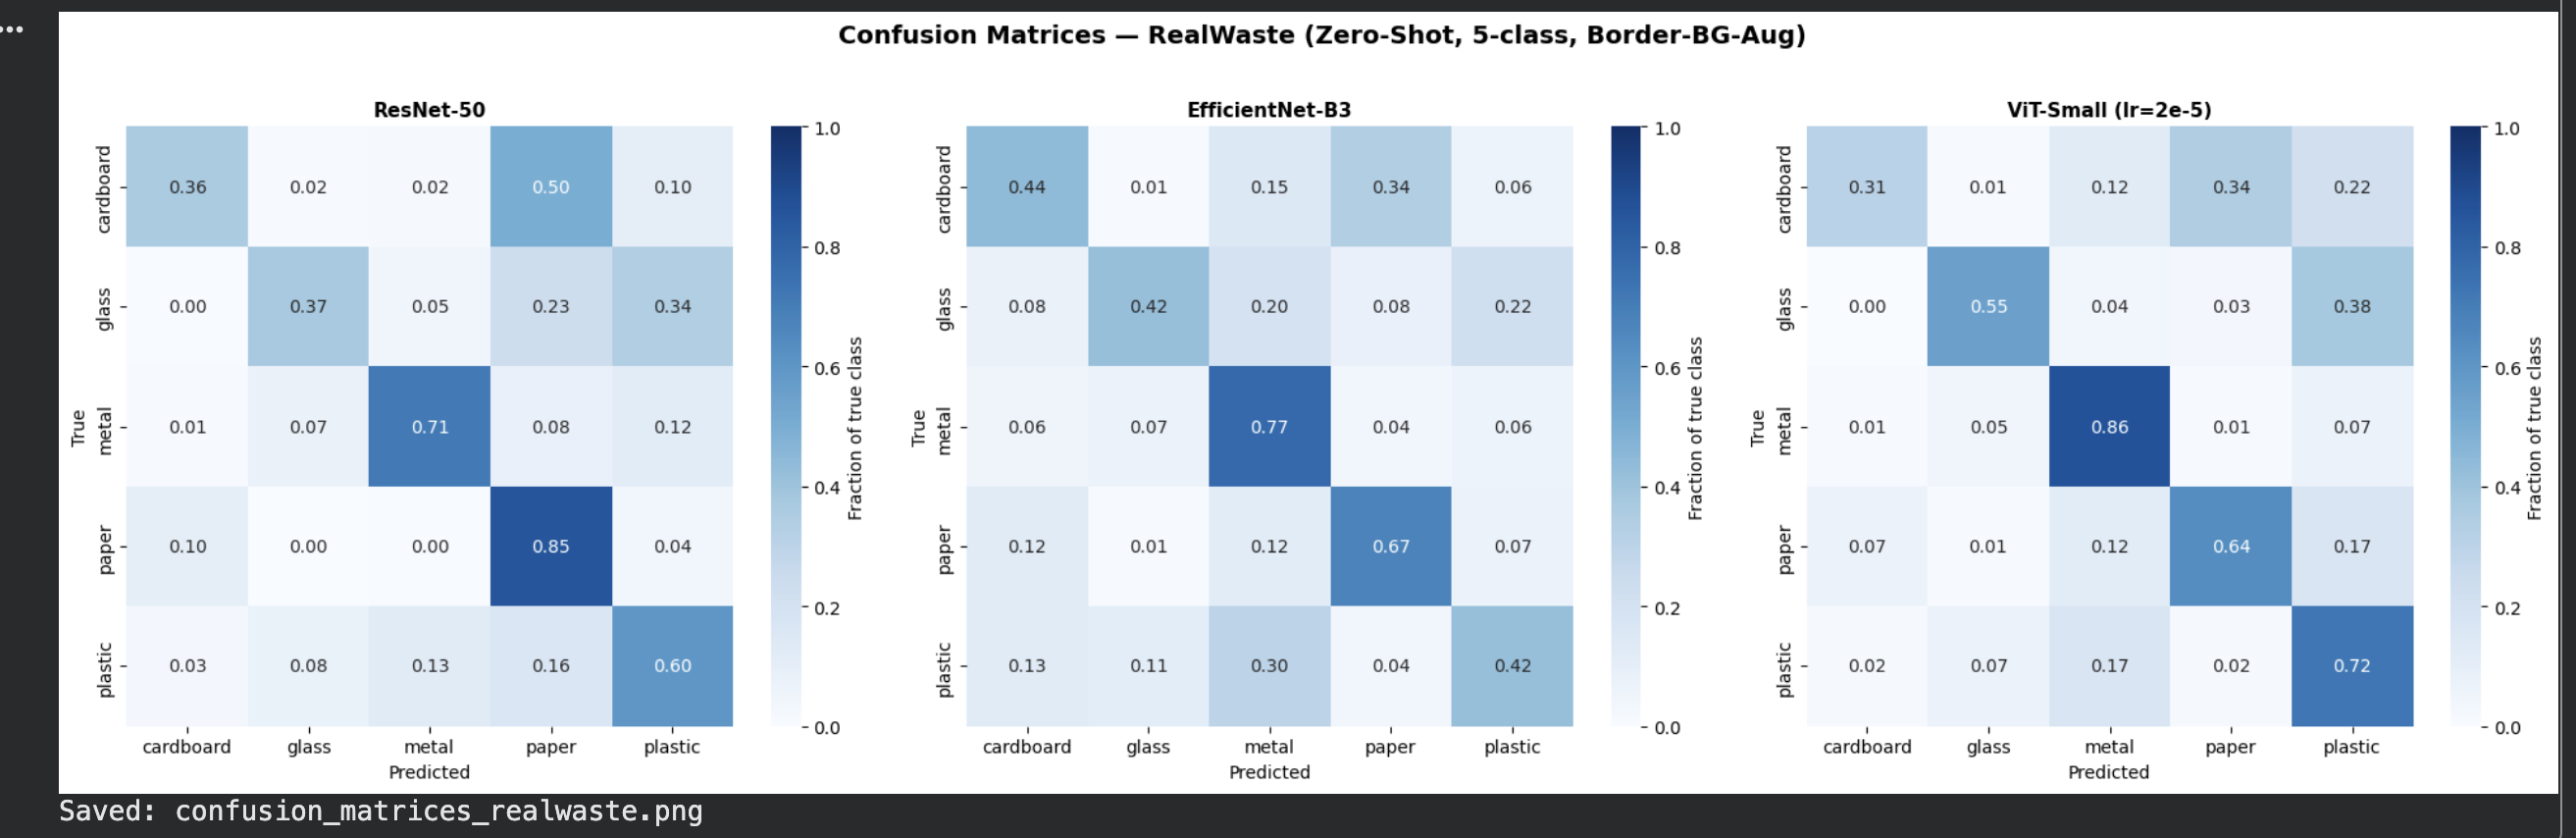
\includegraphics[width=\linewidth]{figures/confusion_matrices_realwaste.png}
\caption{Confusion matrices on RealWaste (5-class, border-background-augmented models). Cardboard$\to$paper and glass$\to$plastic are the dominant, architecture-independent confusions, consistent with genuine material ambiguity in real-world conditions (crushed/wet cardboard resembling paper; broken or clear glass resembling plastic) rather than model-specific weaknesses.}
\end{figure}

\end{document}
